\section{Introduction}

Photosensor Test Facility

What is the PTF? 




As discussed in the previous sections, many of PMT properties can be
calibrated {\it in-situ} by deploying several calibration sources in
the detector.
%
We will have additional {\it ex-situ} measurements to understand
further details of PMT properties that are difficult to measure
in-situ.

A number of PMTs that are installed into Hyper-K must first be
precalibrated to allow the gain of the detector to be tuned for
uniformity. The charge recorded per photoelectron is a function of the
high voltage applied to the PMT and of the PMT itself. It is important
to characterise the response of a number of PMTs that are installed
uniformly into the detector. Using these known PMTs once the detector
is running, the high voltage applied to each PMT will be tuned such
that each PMT has the same gain. In Super-K 420 PMTs were
precalibrated using a Xe lamp connected via an optical fibre to a
scintillator ball in a shielded dark box in which the PMT to be
calibrated was mounted.

%It is known that a 
Large photo-cathode area PMTs have non-uniform charge and time
responses.  The photo-detection efficiency for example can vary
depending on the photon incident angle and position on the
photo-cathode of the PMT (e.g. \cite{Goon:2012if}).
%
Such non-uniformity of PMT responses need to be understood and are
required to build a better model of PMT responses, which is then
adopted in the detector simulation.
%
There are some difficulties to measure such non-uniformity of PMT
responses after they are installed in the detector since, for example,
a small non-uniformity of water transparency can make an apparent
variation of PMT responses.
%
Thus, we need to establish a special test stand for the measurements.
%

A test facility, called `photosensor test facility (PTF),' has been
built at TRIUMF.  Figure~\ref{fig:calib_PTF} shows a photograph and
schematic diagram of PTF.
%
\begin{figure}[htbp]
  \begin{center}
  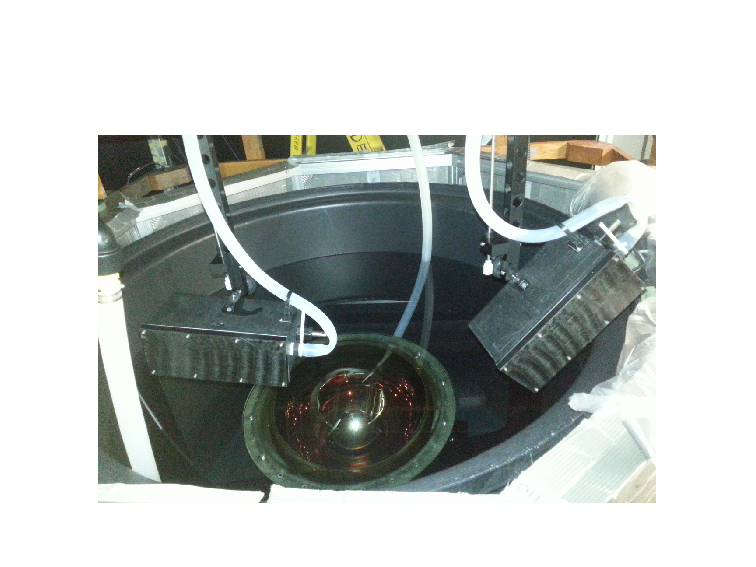
\includegraphics[width=0.55\textwidth]{calib_PTF_photo.pdf}
  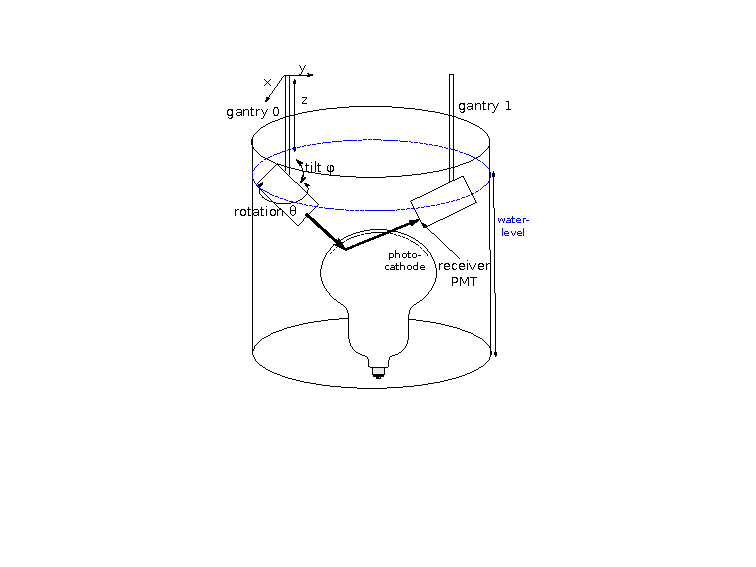
\includegraphics[width=0.35\textwidth]{calib_PTF_schematic.pdf}
  \caption{Photograph (left) and schematic diagram (right) of the photosensor test facility
    at TRIUMF.}
  \label{fig:calib_PTF}
  \end{center}
\end{figure}
%
The PTF has two manipulator arms (gantries) which are motorized and
move independently in the $x$-, $y$-, $z$-direction, rotation, and
tilt.  Each gantry is equipped with an optical box that contain a
light source with a chosen wavelength, a (monitor) PMT to measure the
intensity of the injected light and a (receiver) PMT which is used for
measurement of reflectivity.  The PTF is equipped with a water
purification system, which generates ultra-pure water, and can measure
PMT responses under water.
%
As discussed in the photosensor section, Hyper-K PMT will be
completely encased in a pressure housing.  The optical properties of
the PMT housing in ultra-pure water will also be measured by the PTF.
%
Currently, characterization of the 20-inch SuperK PMT is under way at PTF.
The ambient magnetic field is compensated down to 5mG level by a three sets
of Helmholtz coils and the desired magnetic field can be applied to study the
impact of the ambient magnetic field (Figure~\ref{fig:PTF_field}). Five milli-meter grid 
scan on the SK PMT photocathode revealed significant gain variation due to the 
venetian blind dynode structure. Significant gain variation due to the magnetic field 
is also observed (Figure~\ref{fig:SKPMT_PTF}). 
%
\begin{figure}[htbp]
  \begin{center}
  \begin{tabular}{c}
  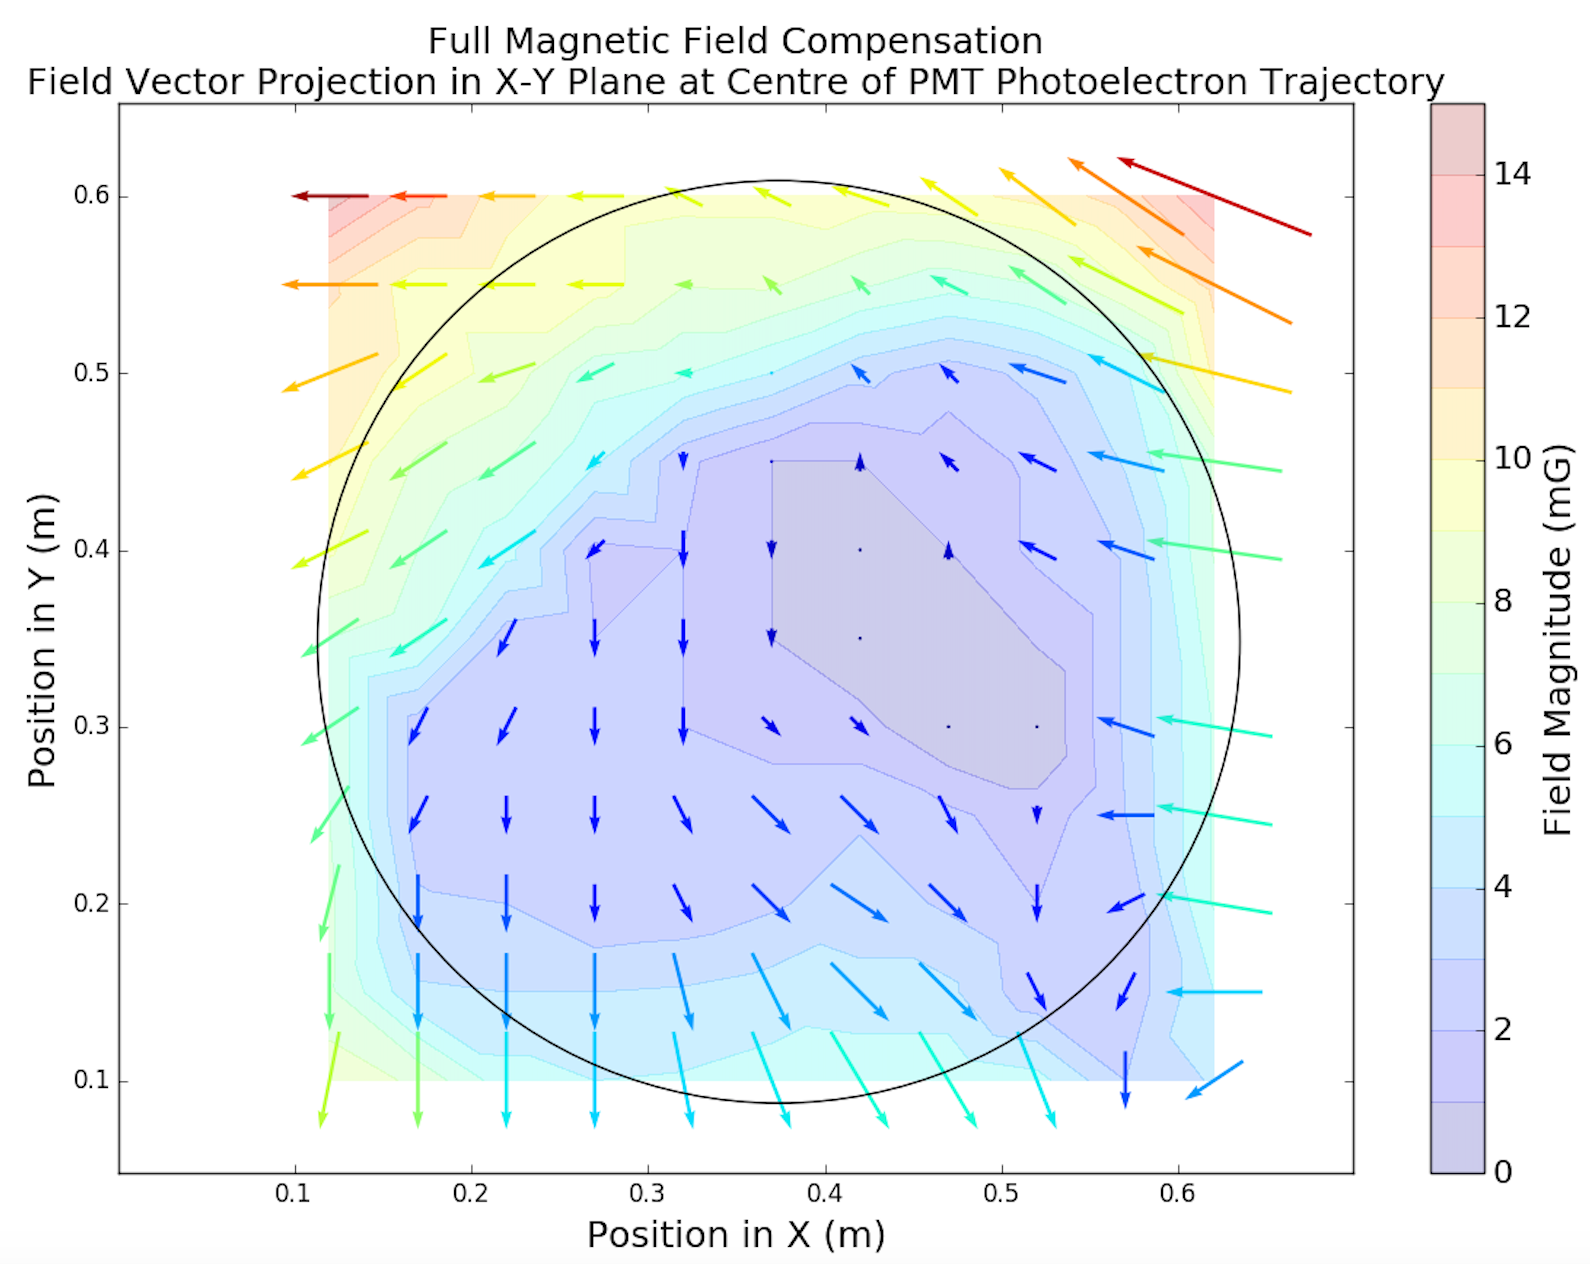
\includegraphics[width=0.65\textwidth]{calib_PTF_field_1.png} \\
  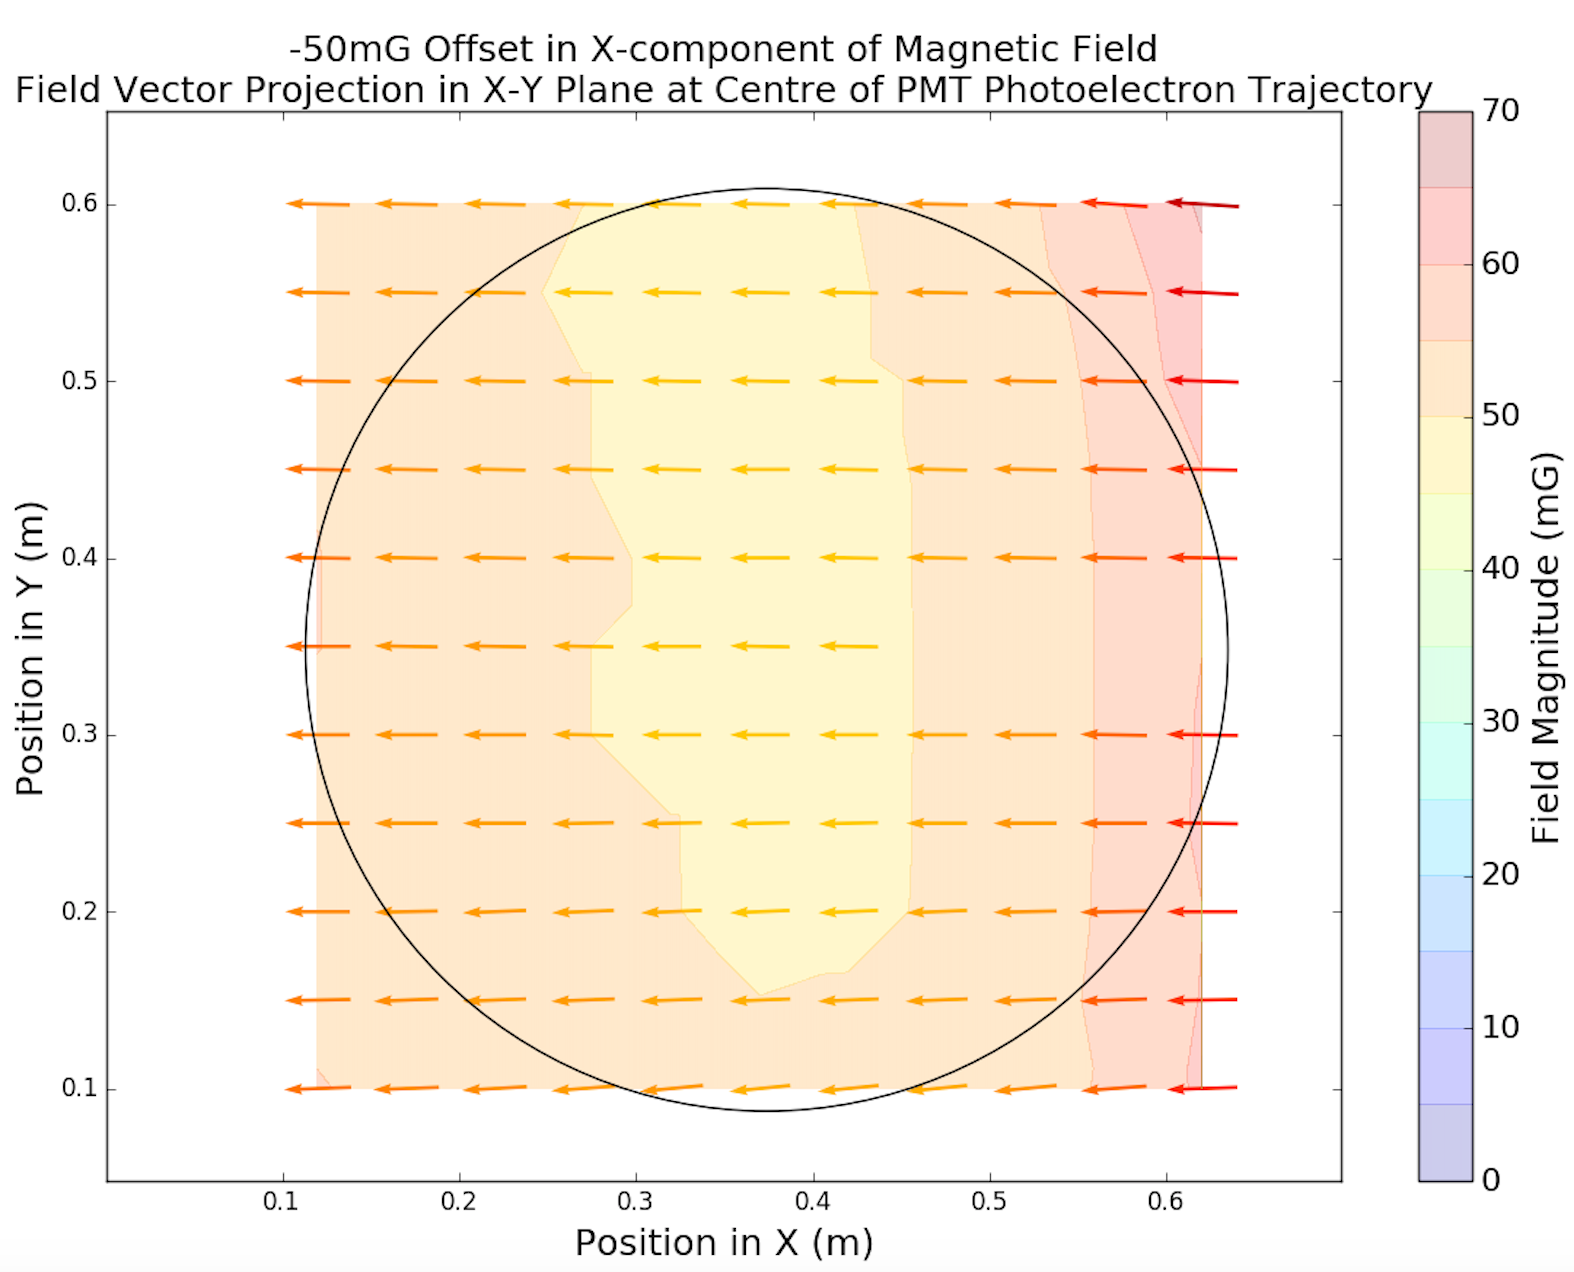
\includegraphics[width=0.65\textwidth]{calib_PTF_field_3.png} \\
  \end{tabular}
  \caption{Map of the compensated magnetic field at PTF (top) and 
 with 50mG field in the -x direction  (bottom).}
  \label{fig:PTF_field}
  \end{center}
\end{figure}
%
%
\begin{figure}[htbp]
  \begin{center}
  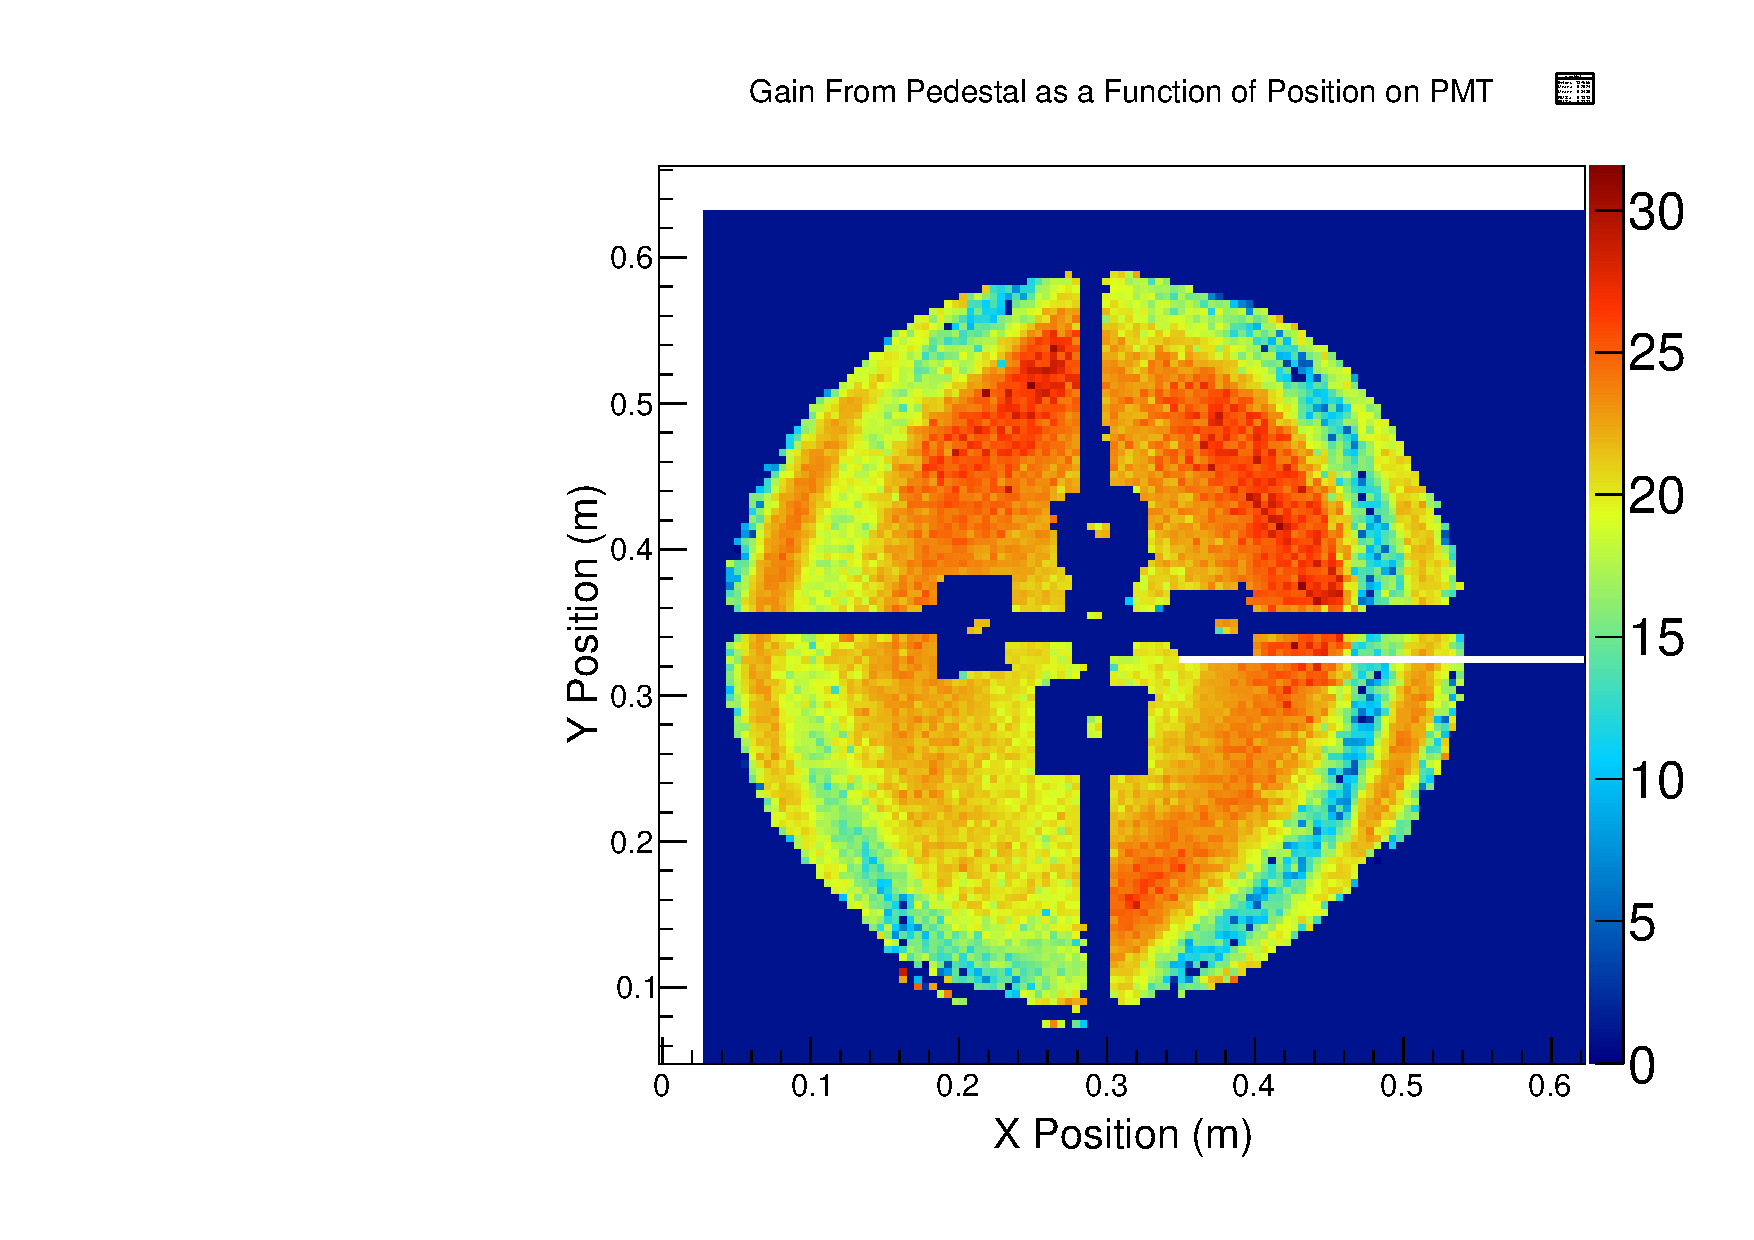
\includegraphics[width=0.6\textwidth]{calib_PTF_SKPMT.pdf}
  \caption{SK-PMT gain distribution under fully compensated field. The low gain valley
  comes from the photoelectrons escaping the first stage of the venetian blind dynode. 
  Also visible in the figure is the affect of adhesive tape applied to the PMT to allow 
  precise determination of position and orientation of the system.}
  \label{fig:SKPMT_PTF}
  \end{center}
\end{figure}
%

Calibration of the SK PMT along with the establishment of the PMT characterization procedure
at PTF will continue till the end of 2017. From 2018, PTF will focus on the characterization of
mPMT prototype for NuPRISM and Hyper-K and the final version of the 20-inch B\&L PMT for 
HyperK. From 2019 PTF will focus on the design study of mPMT for NuPRISM, and then test
the sampled modules for NuPRISM production. From 2022, PTF will test sampled 
photosensors for HyperK production till the end of 2024 when the HyperK photosensor installation 
starts.

In addition to PMT studies at the PTF facility, measurements of
Super-K PMT properties continue at Kamioka. Initial measurements from
these studies are complete and have been implemented into
SKDETSIM. The impact of these measurements on physics analyses are
ongoing.



% Q3/16 - Q3/17  Establishment of 20-inch PMT characterization method using SK PMT
% Q4/17 - Q4/18  Characterization of mPMT and B&L PMT
% Q1/19 - Q2/20  Study for mPMT designs for NuPRISM and HK
% Q3/20 - Q4/21  mPMT study for NuPRISM production
% Q1/22 - Q4/24  mPMT and B&L studies for HK production
